\section{FMCW Primer}\label{sec:fmcw}
Frequency Modulated Continuous Wave (FMCW) radar technology is a range and velocity measuring technique, in which transmitter transmits a frequency modulated chirped signal and the receiver uses the frequency shift between the transmit signal and the received signal to estimate the range.  


\begin{figure}[h!t]
%\vspace{-0.1in}
\center{
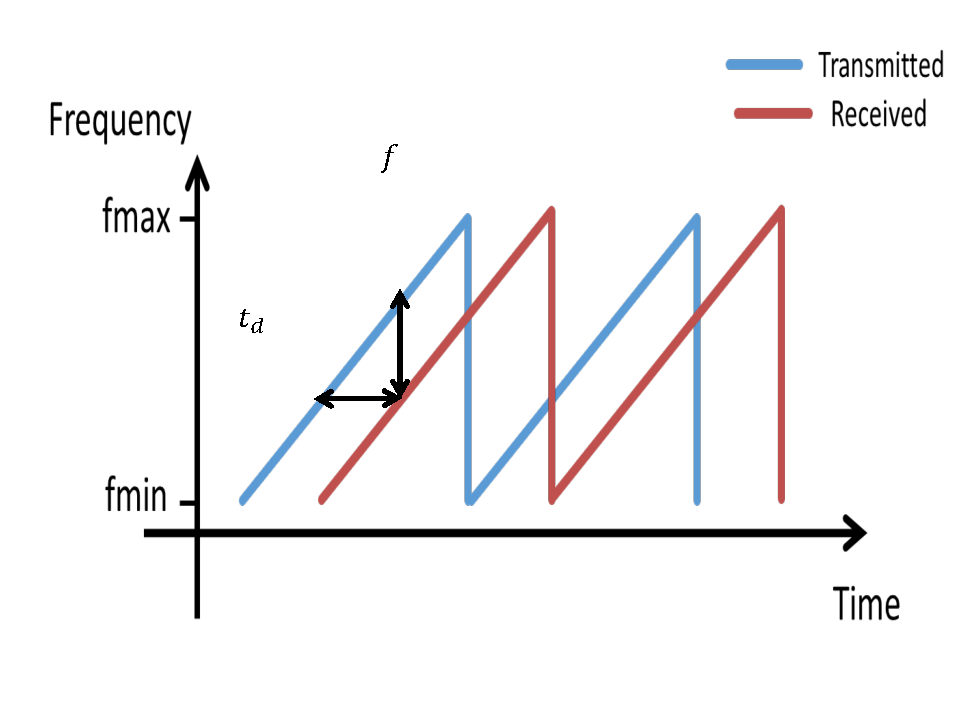
\includegraphics[width=0.3\textwidth]{figs/fmcw.pdf}
%\vspace{-0.1in}
\caption{{\small FMCW in action}}
%\vspace{-0.1in}
\label{fig:fmcw}
}
\end{figure}

In our setup we have co-located speaker and microphone. The speaker transmit an FMCW chirp periodically as shown in Figure XXX. The frequency of the signal sweeps linearly from $f_{min}$ to $f_{max}$ in each period. The frequency within each sweep is $f = f_{min} + \frac{Bt}{T}$ , where B is the signal bandwidth, T is the sweep time. Integrating the frequency over time gives us phase of the signal: $u(t)=2 \pi (f_{min}t + B \frac{t^2}{2T} )$.
Thus giving the transmitted signal during the n-th sweep to be
$$v_t(t') = cos(2 \pi f_{min}t'  + \pi B\frac{t'^2}{T})$$ where $t' = t - nT$ .

Lets consider the transmitted chirp signal is reflected by the object and arrives at the receiver after a delay $t_d$. The received signal is attenuated and delayed in time, and becomes:
$$v_r(t) = \alpha cos(2 \pi f_{min}(t - t_d) + \frac{\pi B(t - t_d)^2}{T} )$$
where $\alpha$ is the attenuation factor.

The receiver mixes (i.e., multiplies) the received signal with the transmitted signal. That is, $v_m(t) = v_r(t)v_t(t)$. Thus, $v_m(t)$ is a product of two cosines. By using $cos A cos B = (cos(A - B) +
cos(A + B))/2$ and filtering out the high frequency component $cos(A + B)$, $v_m(t)$ becomes:
$$ v_m(t) = \alpha cos(2 \pi f_{min} t_d +
\pi \frac{B(2 t_d t - t_d^2)}{T} ).$$
Suppose the mobile is at distance $\frac{R}{2}$ from the reflecting object, reflection from that object would propagate a distance of $R$ before it is received by the microphone, so $t_d$ is given by $(R)/c$. Plugging $t_d$ into signal above, gives us
$$v_m(t) = \alpha cos(2 \pi f_{min} \frac{R}{c} + 2 \pi Bt\frac{R}{cT} - \pi B\frac{R^2}{c^2 T} ))$$.

To analyze the frequency components of the above mixed signal we take derivative of its phase, the constant term can be ignored and the terms quadratic with respect to $1/c^2$ are too small and
can also be ignored. The remaining frequency component, denoted as fp comes out to be:
$$f_p = \frac{1} {2\pi} \frac{\delta Phase}{\delta t} = \frac{BR}{cT}$$
This means that the frequency spectrum of the mixed signal will have a peak at $\frac {BR}{cT}$. If there are multiple propagation paths between the transmitter and the receiver, multiple peaks are observed in the FFT spectrum of the mixed signal. 
Based on observed $f_p$ in the FFT spectrum, the distance R can be derived as:
$$R = \frac{f_pcT}{B}$$ .

xxx need changes xxx
In our set up, before being transmitted the FMCW chirp is shaped by passing it through a window. Shaping the chirp improves the its signal-to-noise ratio by improving the peak-to-sidelobe ratio. 
The chirp signal is windowed using a hanning window XXX ref. The hanning window is described by
\begin{equation}H[n] = 0.5{\ast}\left(1-{\rm{ cos}}\left(\frac{2{\ast}\pi{\ast}n}{N-1}\right)\right).\end{equation}
The discretized pulse is shaped by performing an element-wise multiplication between the discretized pulse vector and the discretized hanning window. Finally, the discretized shaped pulse is sent to the speaker’s buffer to be transmitted
%\begin{figure}[hbt]
%  %\vspace{-0.15in}
%\centering{
%\subfigure[]{
%    \fbox{\includegraphics[width=0.40\columnwidth, %keepaspectratio]{figs/anechoic_experiment.jpg}}
%    \label{fig:anechoic}
%}
